\section{Anhang}
\subsection{Quellcode}\label{Quellecode}
Der komplette Code der Anwendung befindet sich im Githubprojekt.\\
Link: \url{https://github.com/hebelsan/OpenPearl-Semesterprojekt/tree/master/Project}\\
In diesem Ordner befinden sich zwei Programme.\\
Ein Programm mit neu entwickelten Ausgabe und ein Programm ohne bearbeitet Ausgabe.\\
\subsection{Abgeändertes OpenPearl-Projekt}\label{abgeänderte OpenPearl-Projekt}
Das von uns abgeänderte OpenPearl-Projekt befindet sich unter folgendem Link.\\
\url{https://github.com/hebelsan/OpenPearl-Semesterprojekt/tree/master/openpearl}\\
\subsection{Aktivitätsdiagramm}\label{Aktivitätsdiagramm}
Das Aktivitätsdiagramm befindet sich ebenfalls im Repository unter \url{https://github.com/hebelsan/OpenPearl-Semesterprojekt/tree/master/docs/Activity_Diagram}.\\
\newpage
\subsection{Änderungen der Makefile im Ordner runtime}\label{Änderungen der Makefile im Ordner runtime}
\begin{figure}[h]
\begin{center}
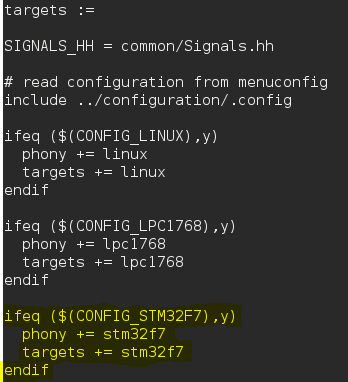
\includegraphics[width=9cm]{grafiken/Makefile_runtime1.png}
\end{center}
\end{figure}
\clearpage
\begin{figure}[h]
\begin{center}
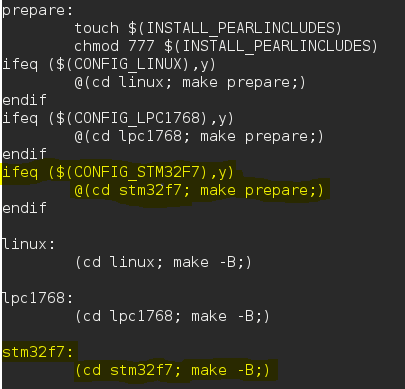
\includegraphics[width=11cm]{grafiken/Makefile_runtime2.png}
\end{center}
\end{figure}

\begin{figure}[h]
\begin{center}
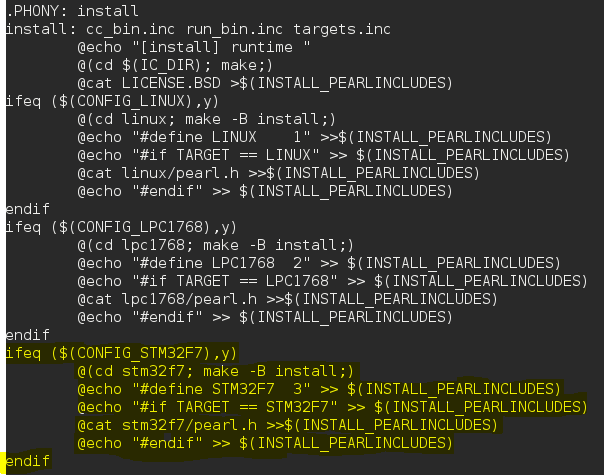
\includegraphics[width=15cm]{grafiken/Makefile_runtime3.png}
\end{center}
\end{figure}
\clearpage
\begin{figure}[h]
\begin{center}
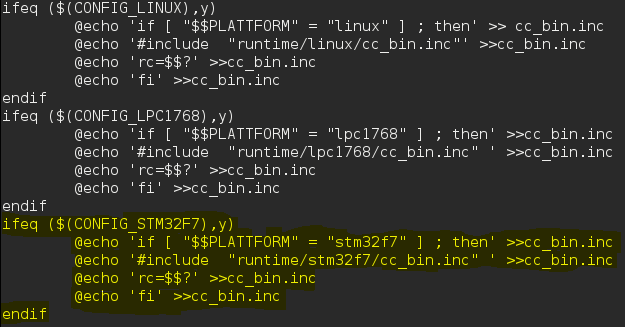
\includegraphics[width=16cm]{grafiken/Makefile_runtime4.png}
\end{center}
\end{figure}

\begin{figure}[h]
\begin{center}
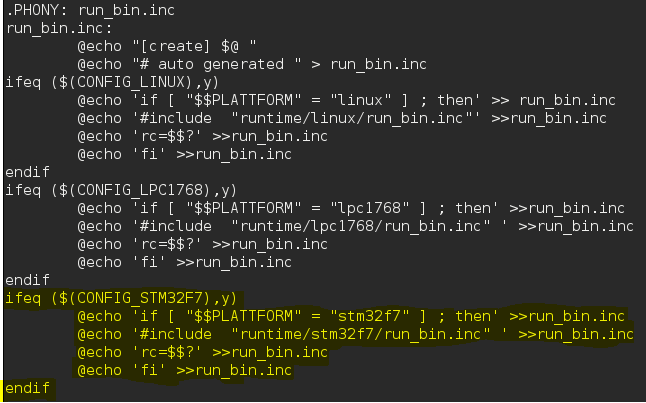
\includegraphics[width=16cm]{grafiken/Makefile_runtime5.png}
\end{center}
\end{figure}
\clearpage
\subsection{Änderungen der Makefile im Ordner stm32f7}\label{Änderungen der Makefile im Ordner stm32f7}
\begin{figure}[h]
\begin{center}
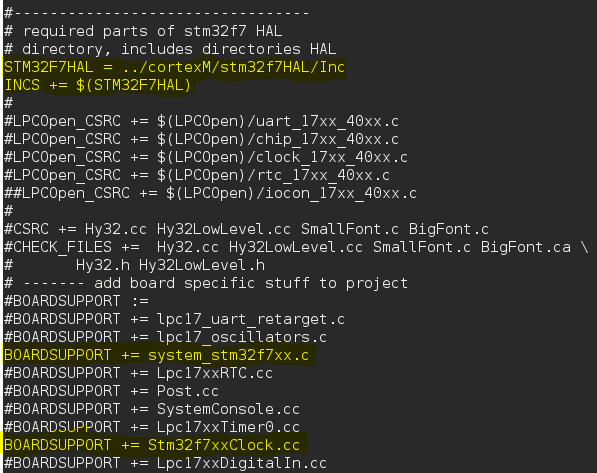
\includegraphics[width=13cm]{grafiken/Makefile_stm32f7_1.png}
\end{center}
\end{figure}

\begin{figure}[h]
\begin{center}
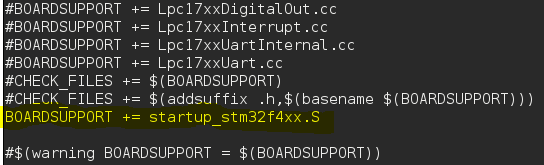
\includegraphics[width=13cm]{grafiken/Makefile_stm32f7_2.png}
\end{center}
\end{figure}
\newpage

\begin{figure}[h]
\begin{center}
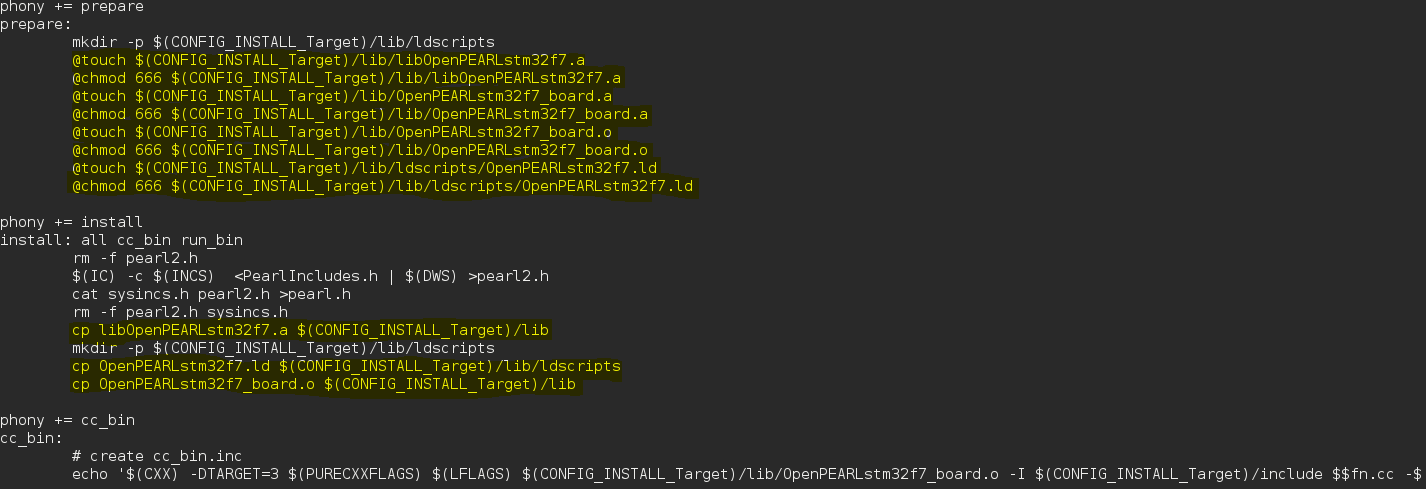
\includegraphics[width=35cm]{grafiken/Makefile_stm32f7_3.png}
\end{center}
\end{figure}

